\documentclass{standalone}

\usepackage{standalone}
\usepackage{tikz}
\usetikzlibrary{er,positioning, calc}

\begin{document}

    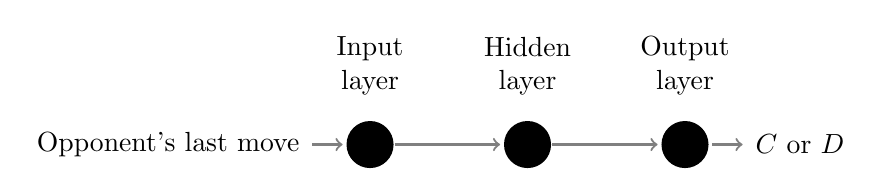
\begin{tikzpicture}[shorten >=1pt,->,draw=black!50, thick]
        \tikzstyle{every pin edge}=[<-,shorten <=1pt]
        \tikzstyle{neuron}=[circle,fill=black,minimum size=17pt,inner sep=0pt]
        \tikzstyle{annot} = [text width=4em, text centered]
    
        % Draw the input layer nodes
        \node[neuron, pin=left: Opponent's last move] (0) at (0,0) {};
        
        % Draw the hidden layer nodes
        \node[neuron] (1) at (2, 0) {};
    
        % Draw the output layer node
        \node[neuron,pin={[pin edge={->}]right:\(C\) or \(D\)}] (2) at (4, 0) {};
    
        \path (0) edge (1);
        \path (1) edge (2);
    
        % Annotate the layers
        \node[annot,above of=1, node distance=1cm] (hl) {Hidden layer};
        \node[annot,above of=0] {Input layer};
        \node[annot,above of=2] {Output layer};
    \end{tikzpicture}
\end{document}